%%%%%%%%%%%%%%%%%%%%%%%%%%%%%%%%%%%%%%%%%%%%%%%%%%%%%%%%%%%%%%%%%%%%%%%%%%%%%%%%%%
\begin{frame}[fragile]\frametitle{}

\begin{center}
{\Large Classification in NLTK}
\end{center}
\end{frame}

%%%%%%%%%%%%%%%%%%%%%%%%%%%%%%%%%%%%%%%%%%%%%%%%%%%%%%%%%%%%%%%%%%%%%%%%%%%%%%%%%%
\begin{frame}[fragile]\frametitle{Text Classification}
  \begin{itemize}
    \item Choose the most appropriate label for each piece of text.
    \begin{itemize}
      \item Topic classification
      \item Spam Filtering
      \item Word Sense Disambiguation
    \end{itemize}
  \end{itemize}
\end{frame}

%%%%%%%%%%%%%%%%%%%%%%%%%%%%%%%%%%%%%%%%%%%%%%%%%%%%%%%%%%%%%%%%%%%%%%%%%%%%%%%%%%
\begin{frame}[fragile]\frametitle{Features}
  \begin{itemize}
    \item To decide which label is appropriate for a text, 
      classifiers look at \emph{features} of that text.
    \item Features indicate what aspects of the text are
      relevant for the classification task.
    \item Features are typically hand-crafted for a given task.
  \end{itemize}
\end{frame}

%%%%%%%%%%%%%%%%%%%%%%%%%%%%%%%%%%%%%%%%%%%%%%%%%%%%%%%%%%%%%%%%%%%%%%%%%%%%%%%%%%
\begin{frame}[fragile]\frametitle{Classifying in NLTK}
  \begin{itemize}
    \item Classifiers are applied to \emph{featuresets}:
{\small\begin{lstlisting}
>>> animal = dict(fur=True, legs=4, 
                  size='large', spots=True)
>>> my_classifier.classify(animal)
'leopard'
\end{lstlisting}}
    \item Features are found with a \emph{feature extractor}:
{\small\begin{lstlisting}
>>> def document_features(document):
...     return dict([('contains-word(%s)'%w,True) 
...                  for w in document])
\end{lstlisting}}
    \item Training:
{\small\begin{lstlisting}
>>> train = [(document_features(doc), label)
..           for (doc, label) in labeled_docs]
>>> classifier = NaiveBayesClassifier.train(train)
\end{lstlisting}}
  \end{itemize}
\end{frame}

%%%%%%%%%%%%%%%%%%%%%%%%%%%%%%%%%%%%%%%%%%%%%%%%%%%%%%%%%%%%%%%%%%%%%%%%%%%%%%%%%%
\begin{frame}[fragile]\frametitle{Example: Predict Genders of Names}
  \begin{itemize}
\item Can we guess the gender of the person from name?
\item Observartions: English female names end with $a,e,i$ and mailes with $k,o,r,s,t$
\item Lets build model for this classifiation.
  \item Objective: Given a new name, that we've never seen before, predict
    whether it is male of female.
  \item Use the \texttt{names} corpus.
  \end{itemize}
\end{frame}

%%%%%%%%%%%%%%%%%%%%%%%%%%%%%%%%%%%%%%%%%%%%%%%%%%%%%%%%%%%%%%%%%%%%%%%%%%%%%%%%%%
\begin{frame}[fragile]\frametitle{Steps: Predict Genders of Names}
  \begin{itemize}
\item Step 1: Decide what features of the input are important and how to encode those
\item Final letter of the given name
\begin{lstlisting}
>>> def gender_features(word):
	return {''last letter'': word[-1]}
>>>gender_features('megamind')
{'last letter': 'd'}
\end{lstlisting}
\item Step 2: Prepare training data using names dictionary in nltk
\begin{lstlisting}
>>> from nltk.corpus import names
>>> import random
>>> names = ([name,'male') for name in names.words('male.txt')] +
[name,'female') for name in names.words('female.txt')])
>>> random.shuffle(names)
>>> featuresets  = [(gender_features(n), g) for (n,g) in names]
>>> train_set, test_set = features[500:], features[:500]
\end{lstlisting}
  \end{itemize}
\end{frame}

%%%%%%%%%%%%%%%%%%%%%%%%%%%%%%%%%%%%%%%%%%%%%%%%%%%%%%%%%%%%%%%%%%%%%%%%%%%%%%%%%%
\begin{frame}[fragile]\frametitle{Steps: Predict Genders of Names}
  \begin{itemize}
\item Step 3: Build a classifier from the feature set. Using Naive Bayes
\begin{lstlisting}
>>> classifier = nltk.NaiveBayesClassifier.train(train_set)
>>> classifier.classify(gender_features('Brian'))
>>>'male'
>>> classifier.classify(gender_features('Kathy'))
>>> 'female'
\end{lstlisting}
\item Step 4: Evaluate the classifier in a systematic way on a larger quantity of unseen data, test\_set:
\begin{lstlisting}
>>> nltk.classify.accuracy(classifier,test_set)
>>> 0.774
\end{lstlisting}
  \end{itemize}
\end{frame}

%%%%%%%%%%%%%%%%%%%%%%%%%%%%%%%%%%%%%%%%%%%%%%%%%%%%%%%%%%%%%%%%%%%%%%%%%%%%%%%%%%
\begin{frame}[fragile]\frametitle{Steps: Predict Genders of Names}
  \begin{itemize}
\item Most important features:
\begin{lstlisting}
>>> classifier.show_most_informative_features(5)
Most Informative Features
last_letter = 'a' femaile: male = 34.5 : 1.0
last_letter = 'k' femaile: male = 29.7 : 1.0
last_letter = 'f' femaile: male = 26.5 : 1.0
last_letter = 'v' femaile: male = 10.5 : 1.0
last_letter = 'p' femaile: male = 10.5 : 1.0
\end{lstlisting}
\item Names ending with 'k' are 29.5 times more likely to be male than female
\item Modify \lstinline|gender_features| to add several other features (such as length of names, first letter, etc)
  \end{itemize}
\end{frame}

%%%%%%%%%%%%%%%%%%%%%%%%%%%%%%%%%%%%%%%%%%%%%%%%%%%%%%%%%%%%%%%%%%%%%%%%%%%%%%%%%%
\begin{frame}[fragile]\frametitle{Choosing the right features}
  \begin{itemize}
\item Selecting relevant features is most crucial
\item First, geenrate all the possible features
\item Then check which ones are important.
  \end{itemize}
\begin{lstlisting}
def gender_features2(name):
	features = {}
	features['firstletter'] = name[0].lower()
	features['lastletter'] = name[-1].lower()
	for letter in 'abcdefghijklmnoprstuvwxyz':
		features['count({}).format(letter)] = name.lower().count(letter)
		features['has({}).format(letter)] = (letter in name.lower())
	return features
\end{lstlisting}
\end{frame}


%%%%%%%%%%%%%%%%%%%%%%%%%%%%%%%%%%%%%%%%%%%%%%%%%%%%%%%%%%%%%%%%%%%%%%%%%%%%%%%%%%
\begin{frame}[fragile]\frametitle{IMDB movie reviews dataset}
  \begin{itemize}
\item Source:  http://ai.stanford.edu/~amaas/data/sentiment/
\item Contains 25000 positive and 25000 negative reviews
\item  Contains at most 30 reviews per movie
\item  At least 7 stars out of 10 à positive (label = 1)
\item  At most 4 stars out of 10 à negative (label = 0)
\item  50/50 train/test split
\item  Evaluation: accuracy
  \end{itemize}
\end{frame}

%%%%%%%%%%%%%%%%%%%%%%%%%%%%%%%%%%%%%%%%%%%%%%%%%%%%%%%%%%%%%%%%%%%%%%%%%%%%%%%%%%
\begin{frame}[fragile]\frametitle{Features}
Bag of 1-grams with TF-IDF values
  \begin{itemize}
\item 25000 rows, 74849 columns for training
\item Extremely sparse feature matrix - 99.8\% are zeros
  \end{itemize}
  
  
\begin{center}
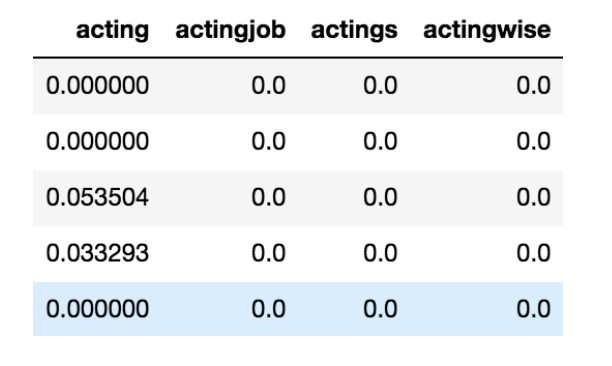
\includegraphics[width=0.6\linewidth,keepaspectratio]{imdb1}
\end{center}
\end{frame}


%%%%%%%%%%%%%%%%%%%%%%%%%%%%%%%%%%%%%%%%%%%%%%%%%%%%%%%%%%%%%%%%%%%%%%%%%%%%%%%%%%
\begin{frame}[fragile]\frametitle{Model}
Logistic regression

$p(y=1|x) = \sigma (w^T x)$
  \begin{itemize}
\item Linear classification model
\item Can handle sparse data
\item Fast to train
\item Weights can be interpreted
  \end{itemize}

\begin{center}
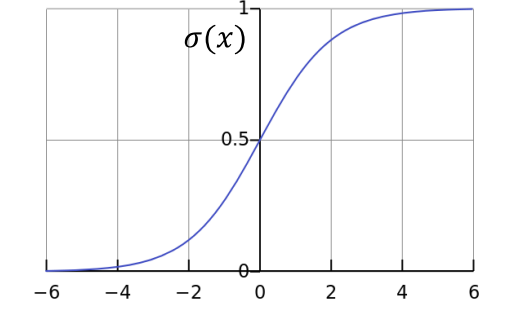
\includegraphics[width=0.6\linewidth,keepaspectratio]{imdb2}
\end{center}
\end{frame}

%%%%%%%%%%%%%%%%%%%%%%%%%%%%%%%%%%%%%%%%%%%%%%%%%%%%%%%%%%%%%%%%%%%%%%%%%%%%%%%%%%
\begin{frame}[fragile]\frametitle{Model}
Results

\begin{itemize}
\item Accuracy on test set: 88.5\%
\item  Let's look at learnt weights:
  \end{itemize}

\begin{center}
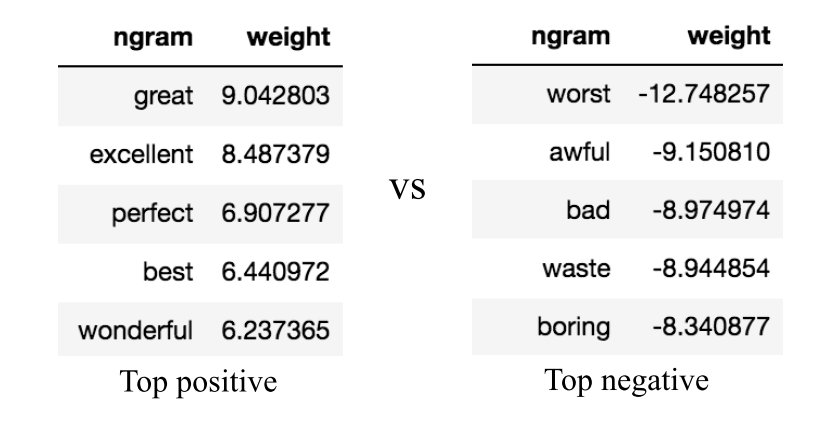
\includegraphics[width=0.8\linewidth,keepaspectratio]{imdb3}
\end{center}
\end{frame}


%%%%%%%%%%%%%%%%%%%%%%%%%%%%%%%%%%%%%%%%%%%%%%%%%%%%%%%%%%%%%%%%%%%%%%%%%%%%%%%%%%
\begin{frame}[fragile]\frametitle{Model}
Let's try to add 2-grams

\begin{itemize}
\item Throw away n-grams seen less than 5 times
\item 25000 rows, 156821 columns for training
  \end{itemize}

\begin{center}
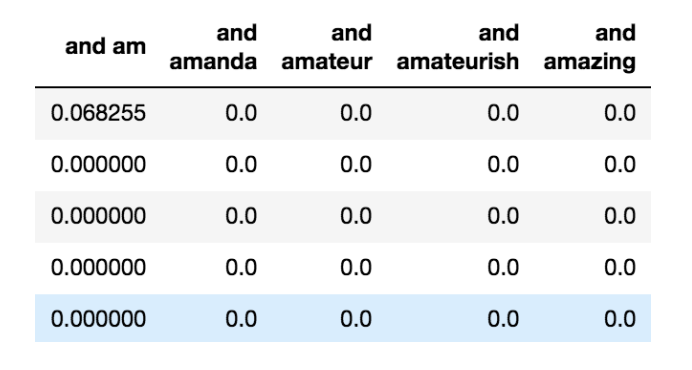
\includegraphics[width=0.8\linewidth,keepaspectratio]{imdb4}
\end{center}
\end{frame}

%%%%%%%%%%%%%%%%%%%%%%%%%%%%%%%%%%%%%%%%%%%%%%%%%%%%%%%%%%%%%%%%%%%%%%%%%%%%%%%%%%
\begin{frame}[fragile]\frametitle{Model}
Results

\begin{itemize}
\item Accuracy on test set: 89.9\% (+1.5\%)
\item Let's look at learnt weights:
  \end{itemize}

\begin{center}
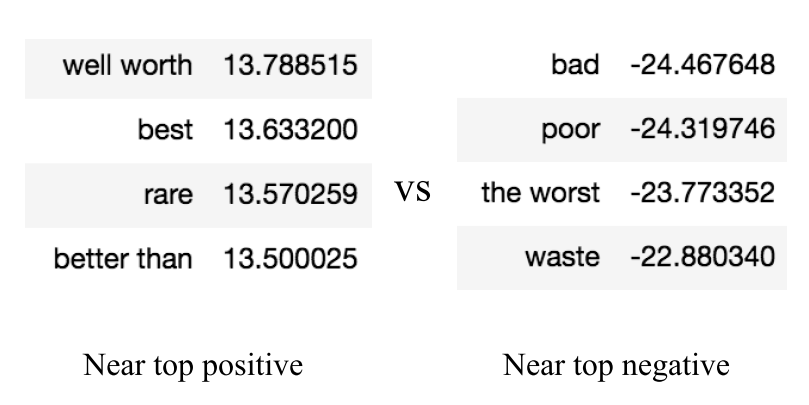
\includegraphics[width=0.8\linewidth,keepaspectratio]{imdb5}
\end{center}
\end{frame}

%%%%%%%%%%%%%%%%%%%%%%%%%%%%%%%%%%%%%%%%%%%%%%%%%%%%%%%%%%%%%%%%%%%%%%%%%%%%%%%%%%
\begin{frame}[fragile]\frametitle{How to make it even better}
Results

\begin{itemize}
\item Play around with tokenization: Special tokens like emoji, '':)'' and ''!!!'' can help
\item Try to normalize tokens: Adding stemming or lemmatization
\item Try different models: SVM, Naïve Bayes, \ldots
\item Throw BOW away and use Deep Learning: 
\begin{itemize}
\item  https://arxiv.org/pdf/1512.08183.pdf
\item Accuracy on test set in 2016: 92.14\% (+2.5\%)
  \end{itemize}
  \end{itemize}

\end{frame}

%%%%%%%%%%%%%%%%%%%%%%%%%%%%%%%%%%%%%%%%%%%%%%%%%%%%%%%%%%%%%%%%%%%%%%%%%%%%%%%%%%
\begin{frame}[fragile]\frametitle{Summary}
Results

\begin{itemize}
\item Bag of words and simple linear models actually work for 
texts
\item  The accuracy gain from deep learning models is not mind 
blowing for sentiment classification
  \end{itemize}

\end{frame}





